% !TEX root = ../main.tex
\subsection{FMT Efficiency}
\label{14.10::fmt_efficiency}
    % Low FMT efficiency + list sources.
    Compared to the alignment work described in Section \ref{12::fmt_alignment_and_reconstruction}, a low FMT is observed in this analysis.
    This is evident in Figure \ref{fig::14.11::vz_seasons}.
    Upon inspection, three causes can be attributed to this: the application of incorrect alignment constants, a geometry effect, and a general FMT offline reconstruction issue.

    In this section, we extensively discussed the efficiency of the FMT detector, addressing alignment issues, as well as the impact of implementing a geometry cut.
    The key findings can be summarised as follows: despite applying corrections, the FMT efficiency for 3-layer tracks remained low, rendering them impractical for exclusive use.
    However, by switching to Spring 2020 data and applying the geometry cut, significant improvements were observed in the detection of trigger electrons and pions.
    Moreover, we thoroughly examined the correlation between efficiency and various variables, namely $v_z$, $\theta$, $\phi$, and $p$.
    The results were as anticipated: strong correlations were observed for $v_z$ and $\theta$, while no significant correlation was found for $\phi$ or $p$.
    These findings provide valuable insights into the performance and limitations of FMT, paving the way for an acceptance correction study and the following work.

    % !TEX root = ../main.tex
\subsubsection{Alignment Effect}
\label{14.11::alignment_effect}
    % Introduction: The problem.
    The data from the RG-F experiment is divided based on the season in which the runs take place, namely Spring 2020 and Summer 2020.
    According to the run group's guidelines, it is recommended to use Summer data as it has undergone more calibration compared to the Spring data.
    However, the calibration work conducted so far does not include the FMT detector, resulting in a significant misalignment effect.

    % Cause of the problem.
    Through simple visual inspection, two distinct peaks can be clearly observed between $z = -36$ cm and $z = -30$ cm in Figure \ref{fig::12.41::dc_vs_fmt_vz_11983}.
    The leftmost peak corresponds to the scattering chamber window, while the second peak corresponds to the RG-F target window.
    These peaks appear merged in Figure \ref{fig::14.10::vz_012933}.
    As discussed in Section \ref{12::fmt_alignment_and_reconstruction}, this issue arises due to the lack of correction for FMT misalignments.

    % Solution.
    The simplest solution is to utilise Spring data.
    Although more calibration work has been performed on the Summer data, it mainly pertains to the CD, which is not used in this analysis.
    Figure \ref{fig::14.11::vz_012016} depicts the same $v_z$ plot from Spring 2020 run 12016, where both peaks are clearly visible.
    This indicates that the misalignment issue has been appropriately addressed in that particular run.

    \begin{figure}[t!]
        \centering\frame{
        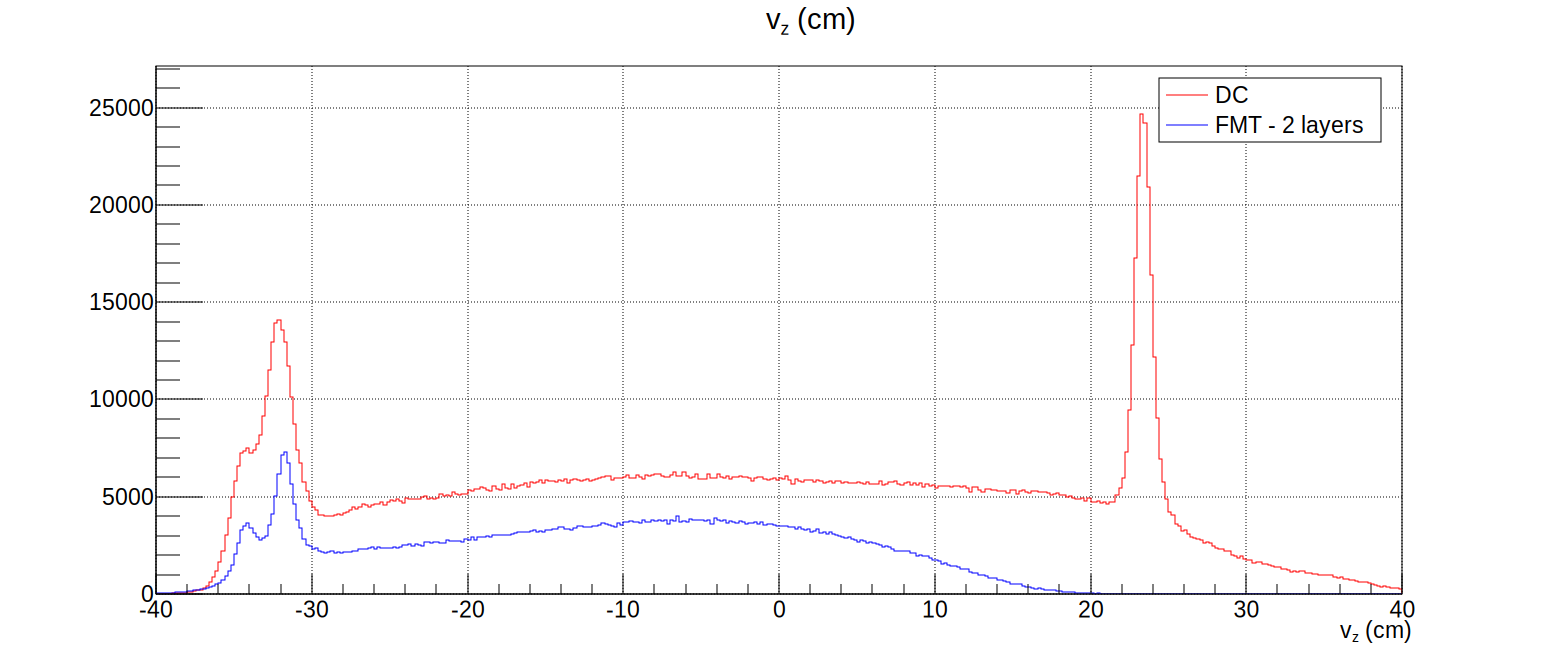
\includegraphics[width=\textwidth]{11vz_012016.pdf}}
        \caption[$v_z$ for DC and FMT, run 12016]{$v_z$ for DC (in red) and FMT (in blue).
        Spring 2020 data, run 12016. The upstream twin peaks can be clearly distinguished, suggesting a correct misalignment correction.
        Source: Own elaboration, using the \href{https://github.com/bleaktwig/clas12-rge-analysis}{clas12-rge-analysis} software.}
        \label{fig::14.11::vz_012016}
    \end{figure}

    % !TEX root = ../main.tex
\subsubsection{Geometry Effect}
\label{14.12::geometry_effect}
    % The effect has already been presented and discussed before, so we're brief.
    This problem has already been extensively discussed in section \ref{12.42::geometry_effect}.
    In summary, the FMT detector is located at approximately $z \approx 26$ cm, and it exhibits poor performance for targets located too close to it.
    The strength of this effect can be quantified by applying the geometry cut described by Equation \eqref{eq::12.42::fmt_geometry_cut} to both the DC and FMT tracks.
    Figure \ref{fig::14.12::vz_012016_geomcut} illustrates the impact of this cut on both the DC and FMT tracks when applied to figure \ref{fig::14.11::vz_012016}.
    The effect of the cut on a $v_z$ vs $\theta$ plot can be observed in Figure \ref{eq::12.42::vz_vs_theta}.

    Based on this cut and the FMT's position along the $z$-axis, subsequent plots will be confined to the range $-30 \text{cm} < v_z < 20 \text{cm}$.

    \begin{figure}[h!]
        \centering\frame{
        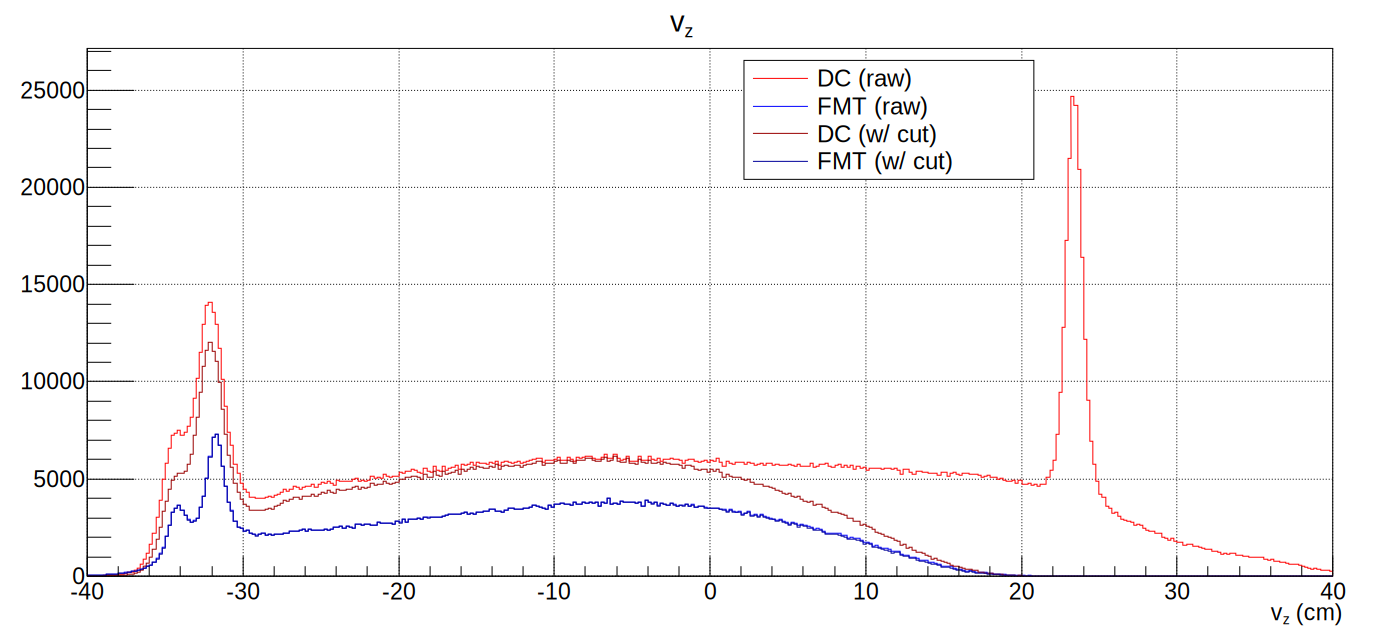
\includegraphics[width=\textwidth]{12vz_012016_geomcut.pdf}}
        \caption[$v_z$ for DC and FMT, w/ and w/out the geometry cut, run 12016]{$v_z$ for DC without the geometry cut (in red), with it (in dark red), for FMT without it (in blue), and with it (in dark blue).
        Spring 2020 data, run 12016.
        The effect is very clear on DC tracks, yet it almost doesn't affect FMT tracks.
        Source: Own elaboration, using the \hyperlink{github.com/bleaktwig/clas12-rge-analysis}{clas12-rge-analysis} software.}
        \label{fig::14.12::vz_012016_geomcut}
    \end{figure}

    % !TEX root = ../main.tex
\subsubsection{Reconstruction Effect}
\label{14.13::reconstruction_effect}
    Even after correcting for both the alignment and geometry issues, the FMT still exhibits lower efficiency compared to what was observed during alignment (compare Figure \ref{fig::14.12::vz_012016_geomcut} with Figure \ref{fig::12.43::dc_vs_fmt_vz_11983_corrected}).
    After conducting a thorough study, it was determined that this effect is not correlated with the run number, beam energy, or beam luminosity.
    Consequently, it can be concluded that the issue is not caused by hardware problems or run conditions.

    Based on these findings, the logical conclusion is that the effect stems from a general issue in the FMT offline reconstruction for data.
    Identifying and rectifying this issue would require a larger project beyond the scope of this thesis and is therefore left as future work.
    For the purposes of this analysis, we will rely on a large number of events to minimize any statistical deficiencies.

    % !TEX root = ../main.tex
\subsubsection{Efficiency Study}
\label{sssec::efficiency_study}
% --+ Integrated. +---------------------------------------------------------
    With all these effects accounted for, we can proceed to study the efficiency in detail.
    First, if we define FMT efficiency as the percentage of DC tracks that get accepted by FMT, we get table \ref{tab::fmt_efficiency_study} for runs 12933 (Summer 2020) and 12016 (Spring 2020).

    \begin{center}
        \begin{tabularx}{0.70\textwidth}{Xr|rrcrr}
            & & \multicolumn{2}{l}{\textbf{Run 12933}}  & & \multicolumn{2}{l}{\textbf{Run 12016}} \\
                             &          & raw  & w/ cut   & & raw  & w/ cut   \\
            \hline
            \textbf{$e^-$}   & 2 layers & 25.1\% & 37.5\% & & 32.7\% & 53.7\% \\
                             & 3 layers &  5.6\% &  8.5\% & &  9.9\% & 16.4\% \\
            \hline
            \textbf{$\pi^+$} & 2 layers &  6.5\% & 13.7\% & & 11.1\% & 28.0\% \\
                             & 3 layers &  0.3\% &  0.7\% & &  1.0\% &  2.7\% \\
            \hline
            \textbf{$\pi^-$} & 2 layers &  5.6\% & 14.2\% & &  8.9\% & 29.5\% \\
                             & 3 layers &  0.3\% &  0.7\% & &  0.9\% &  2.9\%
        \end{tabularx}
        \label{tab::fmt_efficiency_study}
    \end{center}

    % TODO. Change percentages based on new table.
    By switching from Summer to Spring data, we see a $\sim32\%$ increase in trigger electrons detected, and a $\sim36\%$ in all particles.
    Then, by applying the geometry cut in $v_z$ and $\theta$, $\sim64\%$ more trigger electrons are detected (for a $\sim184\%$ total increase), and $\sim126\%$ more particles in general are detected (for a $\sim207\%$ total increase).

% --+ Separated. +----------------------------------------------------------
    We can then check how the efficiency changes as result of the corrections.
    Due to the geometric cut, we expect a strong dependency on $v_z$ and $\theta$, and at most a weak one on $\phi$ and $p$.
    This is what we see in data, as is shown in figure \ref{fig::fmt_efficiencies}.

    % TODO. Explain the loss of dips in $\phi$ efficiency.

    \begin{figure}[t!]
        \centering\frame{
        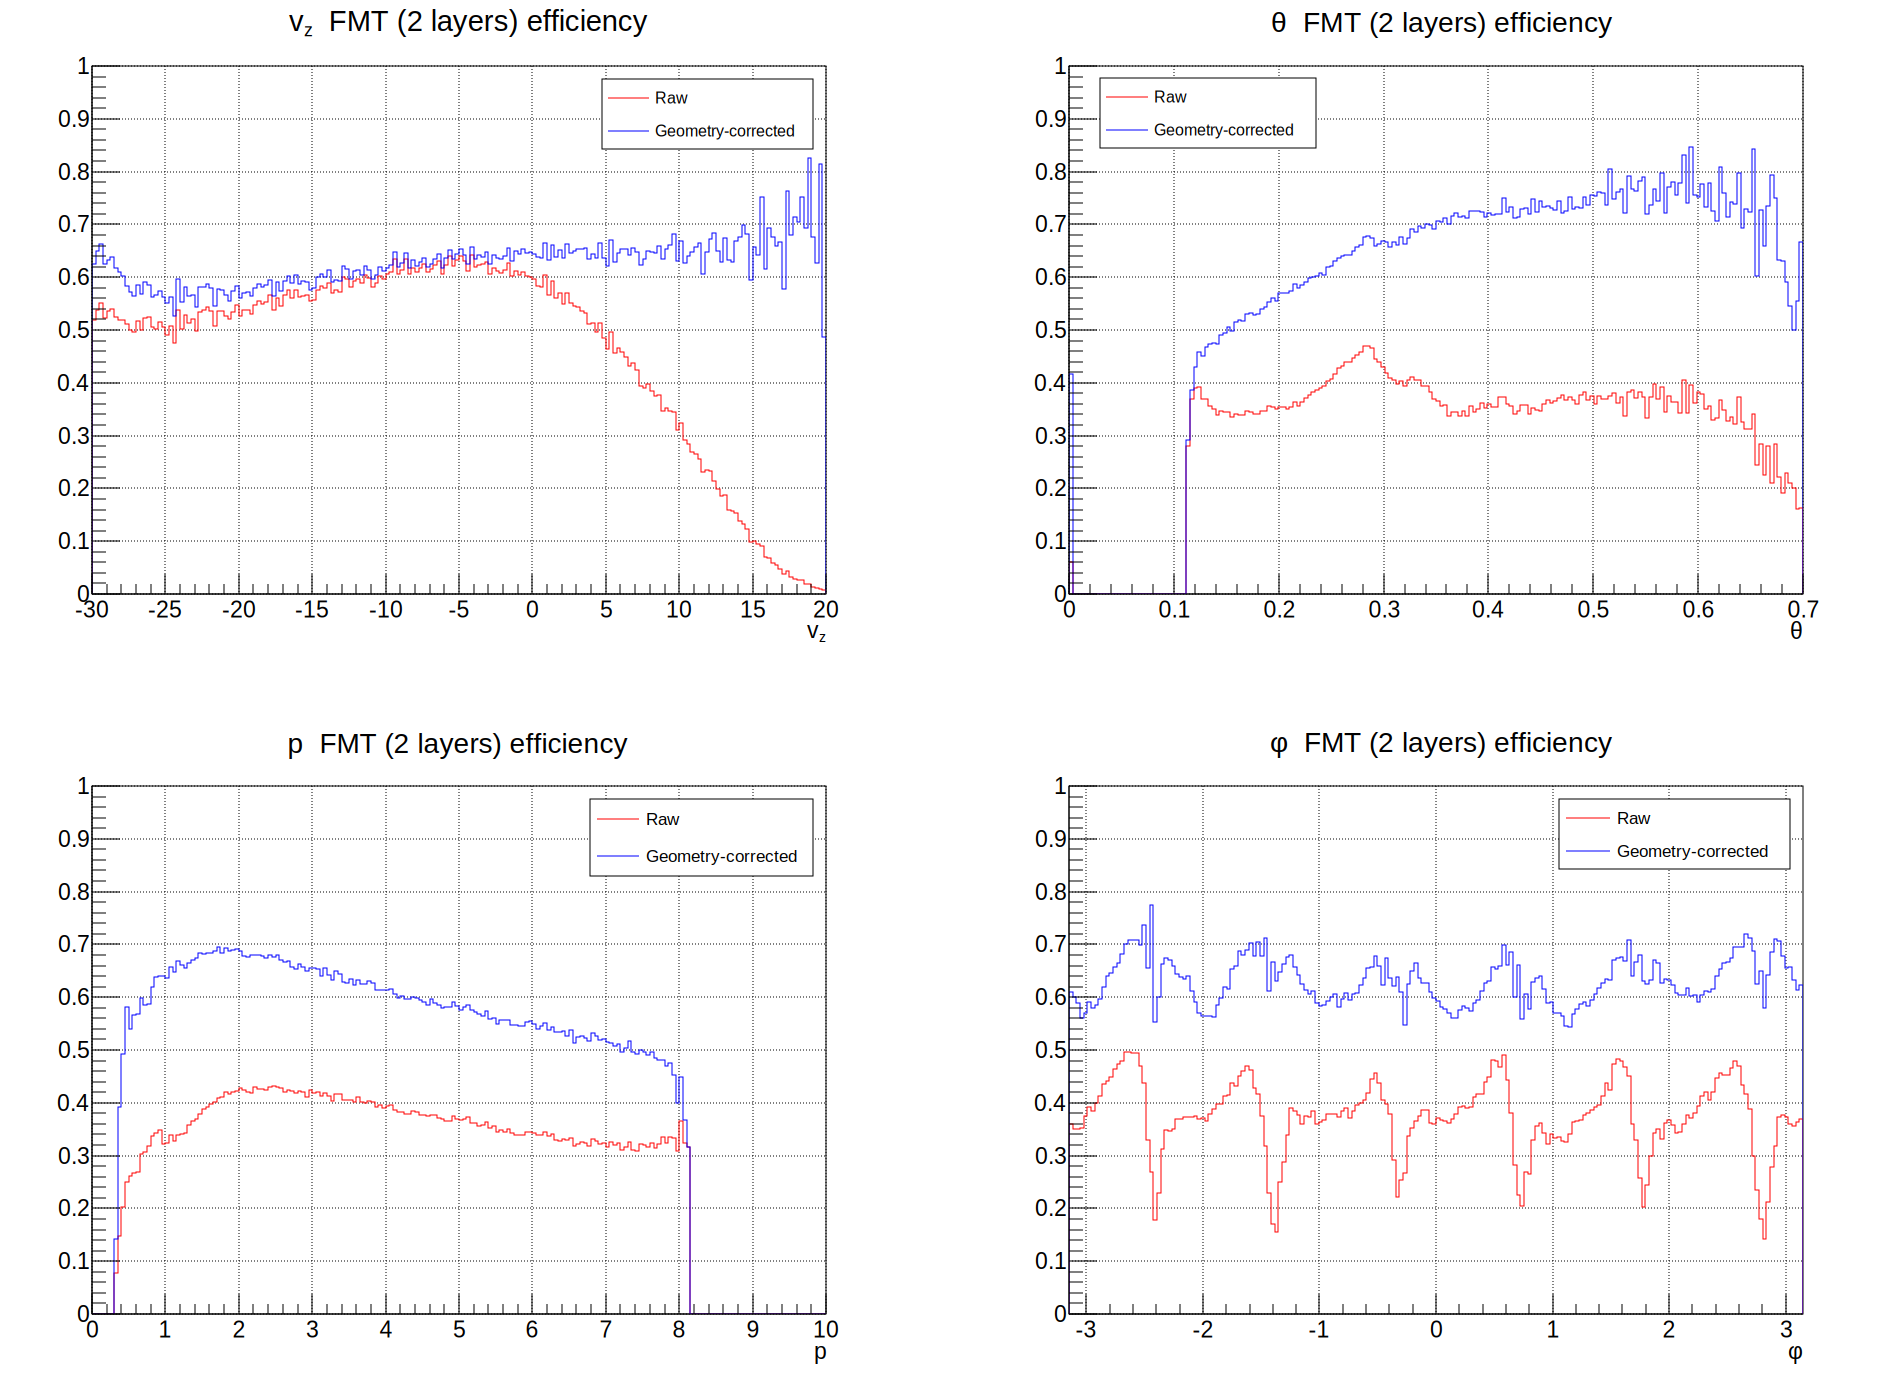
\includegraphics[width=\textwidth]{14efficiencies.pdf}}
        \caption[$v_z$, $\theta$, $\phi$, and $p$ efficiencies for FMT tracks, run 12016]{$v_z$, $\theta$, $\phi$, and $p$ efficiencies for FMT tracks. FMT Efficiency is defined as the percentage of DC tracks that are detected by 2 FMT layers. Run 12016.}
        \label{fig::fmt_efficiencies}
    \end{figure}

